\documentclass[pdftex, 10pt]{IEEEtran}

\usepackage{graphicx}

\DeclareGraphicsExtensions{.png, .jpg}
\graphicspath{{../images/}}

\begin{document}
\title{Computer Exercise 1}
\author{C1C Ian Goodbody\\ECE434\\Dr. York}
\date{\today}
\maketitle

\section{Signal 2}
Signal 2 was composed of $128$ samples of a roughly sinusoidal waveform sampled
at $8000$ Hz. The signal is about $16$ ms in duration. From the time domain waveform, Figure \ref{fig:sig2_td},
one observe at least $2$ component frequencies. The obvious frequency component is at about $1.6$ kHz as determined by
the distance between the peaks. The second component should account for the apparent oscillation of the waveform.

\begin{figure}
    \centering
    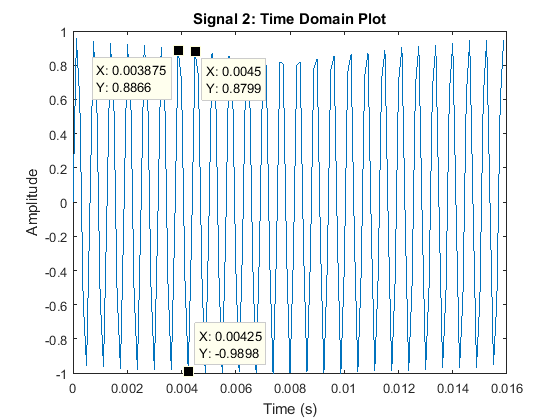
\includegraphics[scale=0.5]{sig2_td}
    \caption{Signal 2: Time Domain}
    \label{fig:sig2_td} 
\end{figure}

The waveform was first transformed to the frequency domain without padding. All waveforms were compared by transforming
them with Rectangular, Bartlett, Hamming, von Hann, and Blackman windows then plotting the linear and decibel magnitudes
of the FFT. 
The Blackman window, Figure \ref{fig:sig2_fd_bm_db_1}, showed two peaks most prominently when plotted with a 
decibel magnitude, the largest at $1.563$ kHz which aligns well with the time domain measurement, 
and one at $2$ kHz. The Blackman window, however, has a fairly broad main lobe width at $0.09375\pi$ which translates
to $375$ Hz and can easily smear signals that are within $188$ Hz. 

\begin{figure}
    \centering
    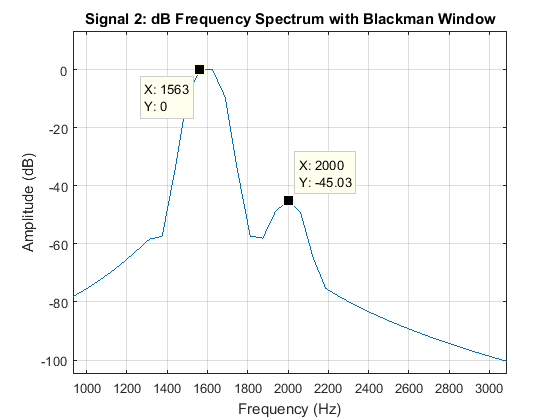
\includegraphics[scale=0.5]{sig2_fd_bm_db_1}
    \caption{Blackman Window, Low Resolution}
    \label{fig:sig2_fd_bm_db_1}
\end{figure}

\subsection{Smearing Analysis}
Padding the windowed waveforms with $128$ extra zeros, then rerunning the transform
and plots, increased the relative frequency resolution from $62.5$ to $31.25$ Hz and better displayed the $2$ kHz
frequency peak across all the windows functions. The higher resolution also made possible smeared peaks more apparent.
Figures \ref{fig:sig2_fd_bm_db_2} and \ref{fig:sig2_fd_hm_db_2} 
show the decibel magnitudes of signal 2 through the Blackman and Hamming windows respectively. The Hamming window,
with a main lobe width of $0.0625\pi$ smearing signals within $125$ Hz, shows three nearly equal peaks around 
$2$ kHz, with a similar perturbation preset in the Blackman windowed waveform. Both the Blackman perturbation at 
$1.875$ kHz and the Hamming perturbation at $1.938$ kHz, are within smearing range for their respective windows.
It is possible that these two perturbations represent a third signal around $1.9$ kHz, but they could also represent
side lobe interference from the $1.59$ kHz with the signal at $2$ kHz.

\begin{figure}
    \centering
    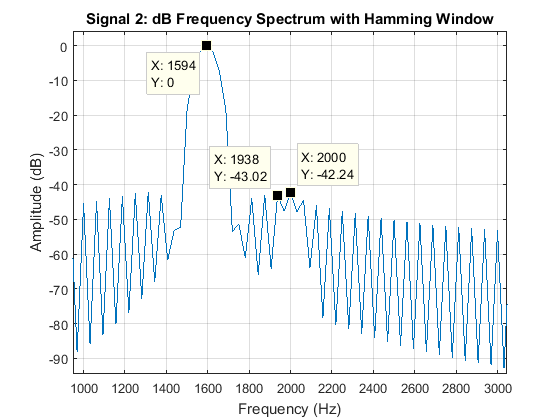
\includegraphics[scale=0.5]{sig2_fd_hm_db_2}
    \caption{Hamming Window}
    \label{fig:sig2_fd_bm_db_2}
\end{figure}

\begin{figure}
    \centering
    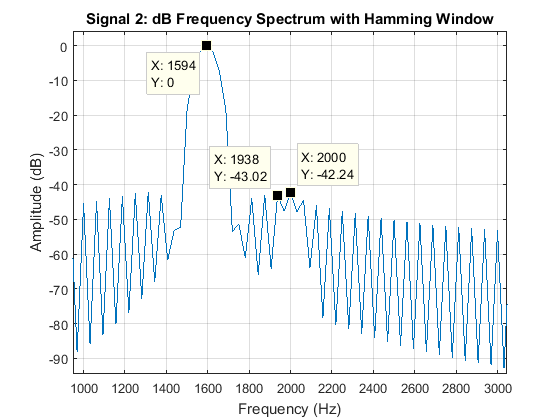
\includegraphics[scale=0.5]{sig2_fd_hm_db_2}
    \caption{Blackman Window, High Resolution}
    \label{fig:sig2_fd_hm_db_2}
\end{figure}

\subsection{Side-Lobe Level Interference}
The possibility of side lobe interference in the Blackman window is fairly low. The side-lobe level between the
main signal at $1.59$ kHz and the secondary signal at $2$ kHz is at $-67.1$ dB. This is far less than $-46.1$ dB 
attenuation between the main and secondary signals so side-lobe level interference is not a factor in 
displaying the $2$ kHz signal. The magnitude possible tertiary signal at or around $1.875$ kHz is $-59.12$ dB
and the side-lobe level at this distance from the $1.59$ kHz peak is $-59.44$ dB. Given the similarity in
attenuations, the perturbation at $1.875$ kHz in the Blackman window is likely the side lobe from the 
main peak smearing with the secondary peak.

The frequency spectrum created by the Hamming window shows three peaks with the tallest centered at $2$ kHz.
With an amplitude of $-42.24$ dB, the amplitude of the secondary signal 
is only slightly greater than the side-lobe level of $-44$ dB. Furthermore, the possible 
tertiary peak at $1.938$ kHz has a gain of $-43.02$ dB which is still greater than the side-lobe level of 
$-43.16$ dB at that distance from the main peak. Given that the secondary peak at $2$ kHz is only slightly
larger than the surrounding side-lobe levels, evidence for the existence of a $2$ kHz signal comes from
the two troughs on either side of the $2$ kHz peak which fall on the theoretical $0$ gain points on the
Hamming window. The levels at these two frequency points do not match the attenuation experienced at
similar $0$ gain points in the waveform. The higher levels at these two troughs are likely due to smearing
around the $2$ kHz peak.

\subsection{Signal 2 Structure}
The most present frequencies in Signal 2 is the main signal at or very near $1.59$ kHz with a
relative amplitude of about $\pm 0.9353$. This amplitude matches the initial time domain analysis
which estimated the frequency at $1.6$ kHz, and it is reasonable to assume that a slight bias from
the secondary signal could draw the $1.59$ kHz closer to $1.6$ kHz. The secondary signal at or near $2$ kHz
has a relative amplitude of about $0.045$, shown in Figure \ref{fig:sig2_fd_rt_ln_2}.

\begin{figure}
    \centering
    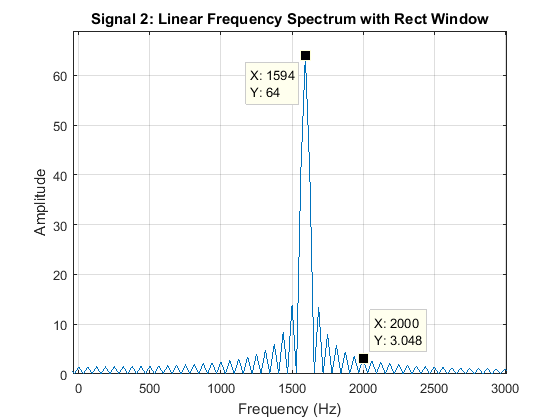
\includegraphics[scale=0.5]{sig2_fd_rt_ln_2}
    \caption{Rectangular Window}
    \label{fig:sig2_fd_rt_ln_2}
\end{figure}

\section{Signal 3}
Signal 3 shown in Figure \ref{fig:sig3_td}, contains what appears to be 3 signals, broadly resembling 
an amplitude modulated wave. The first signal appears to be a carrier frequency distinguished by the
most prominent peaks in the wave. The second signal appears as the envelope waveform shown by the
peaks at $0$ seconds and $0.0125$ seconds. If this second signal is indeed a
modulated signal, then one
would expect to see 2 frequency peaks $80$ Hz on either side of the carrier signal peak.
A third signal, which is difficult to analyze in the 
time domain, appears as the small periodic perturbations in the waveform. The signal itself is $16$
ms long.

\begin{figure}
    \centering
    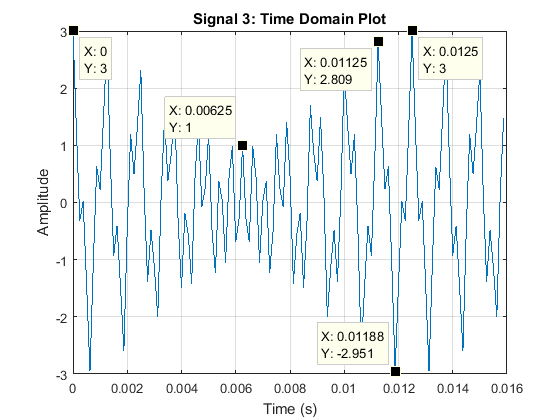
\includegraphics[scale=0.5]{sig3_td}
    \caption{Rectangular Window}
    \label{fig:sig3_td}
\end{figure}

From analysis of the time domain waveform, Figure \ref{fig:sig3_td}, the signals should align 
with $800$ Hz with a relative amplitude of $\pm2.98$ and $80$ Hz with a relative amplitude of $2$.
The third signal cannot be easily be described or estimated using the time domain plot.

\subsection{Smearing Analysis}
Working under the theory that Signal 3 represents an amplitude modulated signal with $2$ peaks
within $80$ Hz of  a larger carrier peak the rectangular window, with a half main-lobe width of 
$62.5$ Hz should provide the necessary resolution without smearing.
Padding the signal to $2$ and $3$ times the original width prior to the applying the FFT, showed
the same 3 peaks. The $3\times128$ length signal is shown in the analysis as the peaks are more
present. The decibel amplitude plot of the rectangular window is shown in Figure \ref{fig:sig3_fd_rt_db_3}.

\begin{figure}
    \centering
    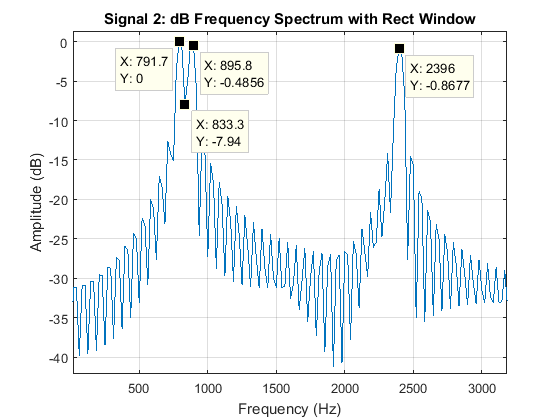
\includegraphics[scale=0.5]{sig3_fd_rt_db_3}
    \caption{Rectangular Window}
    \label{fig:sig3_fd_rt_db_3}
\end{figure}

Three peaks are evident in the plot of the rectangular windowed waveform. Two very close frequency
peaks at $791.7$ Hz and $895.7$ Hz with fairly equal magnitude, then a third peak at $2.396$ kHz
which is slightly shorter than the two main peaks. For comparison, the Hamming and von Hann
window plots data are show in Figures \ref{fig:sig3_fd_hm_db_3} and \ref{fig:sig3_fd_hn_db_3} respectively. 
The frequencies of the three peaks in the are consistent across all three plots, however, 
with main lobe widths of $375$ Hz the trough between the two peaks
is predictably higher in the Hamming and von Hann windows than that gained from 
through Rectangular window. Also the Hamming and von Hann windows show the $2.4$ kHz peak of 
slightly greater amplitude, even though they generally have lower side-lobe levels.

\begin{figure}
    \centering
    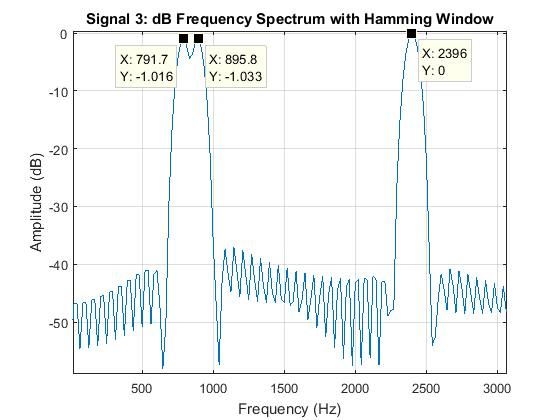
\includegraphics[scale=0.5]{sig3_fd_hm_db_3}
    \caption{Hamming Window}
    \label{fig:sig3_fd_hm_db_3}
\end{figure}

\begin{figure}
    \centering
    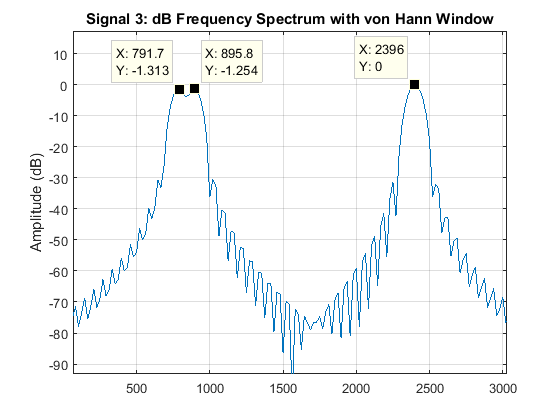
\includegraphics[scale=0.5]{sig3_fd_hn_db_3}
    \caption{Hamming Window}
    \label{fig:sig3_fd_hn_db_3}
\end{figure}

\subsection{Side-Lobe Level Interference}
Comparing Figure \ref{fig:sig3_fd_rt_db_3} with Figures \ref{fig:sig3_fd_hm_db_3} and 
\ref{fig:sig3_fd_hn_db_3} brings up a discrepancy in the respective amplitude of the 
frequency bins. While the von Hann and Hamming windows generally have lower side-lobe levels
than the Rectangular window, both windows the $2.4$ kHz peak higher than the two lower 
frequency peaks. Side-lobe level analysis should indicate which peak is really the highest.

The two peaks on the rectangular window are separated by $104$ Hz corresponding to a 
side-lobe level of $-14.8$ dB which is insignificant relative to the level of the two
peaks. For the $2.4$ kHz peak, side-lobe levels are $-38.2$ dB relative to the $895$ Hz
signal and $-45.4$ relative to the $791$ Hz signal, levels too low relative to the main 
lobe to be very significant in regards to side-lobe level interference.

Analyzing the Hamming window with regards to side lobe interference gives side lobe levels
of $-54.8$ dB and $-61.9$ dB for the $791$ Hz and $895$ Hz signals respectively. These
signals firmly rule out side-lobe level interference, however, because they are much less
than the levels for the rectangular windows, the Hamming and von Hann windows probably give
a better representation of the frequency magnitudes, even if they are all very close.

\subsection{Signal 3 Structure}
In refutation of the AM signal hypothesis, Signal $3$ in Figure \ref{fig:sig3_td} can be best 
represented as a simple addition of $3$ sinusoidal frequencies of roughly equal magnitude at
$791$ Hz, $895$ Hz, and $2.40$ kHz.

\section{Signal 4}
Signal 4 contains $8192$ samples of a fairly complicated and heterogeneous waveform consisting of
lasting a little over $1$ second. The waveform consists of $3$ main noise blocks roughly contained
within times $0.1$ and $0.4$ seconds, $0.45$ and $0.7$ seconds, and $0.7$ and $1$ seconds. Figure
\ref{fig:sig4_td_all} shows the overall time domain plot of the waveform.

\begin{figure}
    \centering
    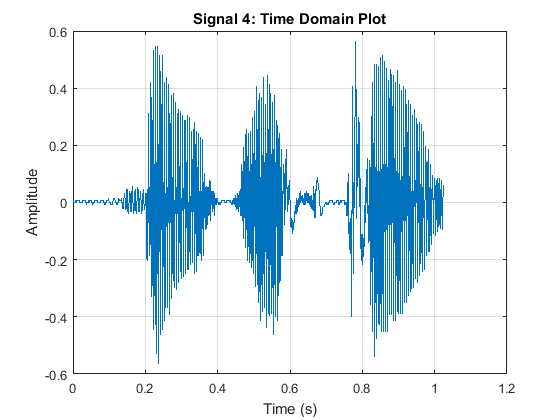
\includegraphics[scale=0.5]{sig4_td_all}
    \caption{Signal 4}
    \label{fig:sig4_td_all}
\end{figure}

A generalized frequency analysis was performed by dividing the waveform into 8 equally sized
blocks, multiplying by a Blackman window, performing the FFT on each blocks, then finally 
averaging the blocks to remove noise. The result is given in figure \ref{fig:sig4_fd_bm_db}. The peaks of the
frequency domain correspond to integer multiples of $160$ Hz, with (roughly) exponentially
decaying peaks. This pattern, albeit with substantial noise, is consistent with several harmonics
of a single note, commonly associated with resonant sounds like musical instruments and the human 
voice box. The fundamental frequency of $160$ Hz should roughly represent the average pitch
of the signal.

\begin{figure}
    \centering
    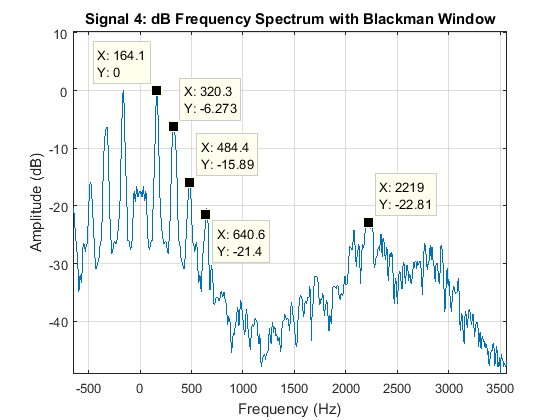
\includegraphics[scale=0.5]{sig4_fd_bm_db}
    \caption{Signal 4}
    \label{fig:sig4_fd_bm_db}
\end{figure}

The highly irregular nature of the signal combined with the resonance suggests a human source
for the signal. Indeed listening to the signal as sound showed it as a voice saying the letters
"DSP". Even though the signal well within the bandwidth of the human speaking range, the signal
can still be understood.

\end{document}
